\documentclass[a4paper,12pt]{article}
\usepackage[left=2cm,right=1cm,top=1cm,bottom=1.5cm]{geometry}
\usepackage[utf8]{inputenc}
\usepackage[english,russian]{babel}
\usepackage{graphicx}
\usepackage{amsmath}
\usepackage{amssymb}
\usepackage{cite}
\usepackage{indentfirst}
\usepackage{multicol}
\usepackage{cmap}
\usepackage{hyperref}
\usepackage{esint}
\usepackage{listings}
%\usepackage{minted}
\usepackage{xcolor}
%\usepackage{inconsolata}
%\renewcommand*\familydefault{\ttdefault} %% Only if the base font of the document is to be typewriter style
%\usepackage[T1]{fontenc}
\hypersetup{
	colorlinks=true,
	linkcolor=black,
	filecolor=black,  
	urlcolor=blue,
	pdftitle={Overleaf Example},
	pdfpagemode=FullScreen,
}

\sloppy

\usepackage{geometry}
\geometry{top=2cm}
\geometry{bottom=2cm}
\geometry{left=2.5cm}
\geometry{right=2.5cm}

\renewcommand{\baselinestretch}{1.5}

	\newcommand{\ds}{\displaystyle}
	\renewcommand{\phi}{\varphi}
	\newcommand{\sgn}{\, \text{sgn} \,}
	\renewcommand{\a}{\alpha}
	\renewcommand{\b}{\beta}
	\renewcommand{\l}{\lambda}
	\renewcommand{\d}{\partial}
	\newcommand{\e}{\varepsilon}
	\renewcommand{\^}[2]{#1^{\, #2} \kern -1pt}
	\newcommand{\veco}{\kern -1pt \vec{\kern 1pt 0}}
	\newcommand{\1}{\kern 1pt}
	\newcommand{\0}{\kern -1pt}
	%\renewcommand{\Phi}{\varPhi}
	
\newcommand{\vs}{\vspace{0.2cm}}
	
	
\begin{document}
	
	\begin{titlepage}
		\begin{center}
			\small{Национальный исследовательский ядерный университет «МИФИ»}\\*
		\end{center}
		\vspace{7cm}
		
		\begin{center}
			\Large{\textbf{Задание по курсу}\\
				\textbf{«Теория управления»}}
		\end{center}
		\vspace{2cm}
		
		\begin{flushright}
			Выполнил\\
			студент группы Б21-215\\
			Рокин Олег Дмитриевич\\
			\vspace{0.5cm}
			Вариант №6
		\end{flushright}
		\vspace{8cm}
		
		\begin{center}
			\textbf{2023}
		\end{center}
	\end{titlepage}


	\newpage 
	\setcounter{page}{2}
	
	
	Исходная структурная схема линейной динамической системы:
	
	\begin{center}
		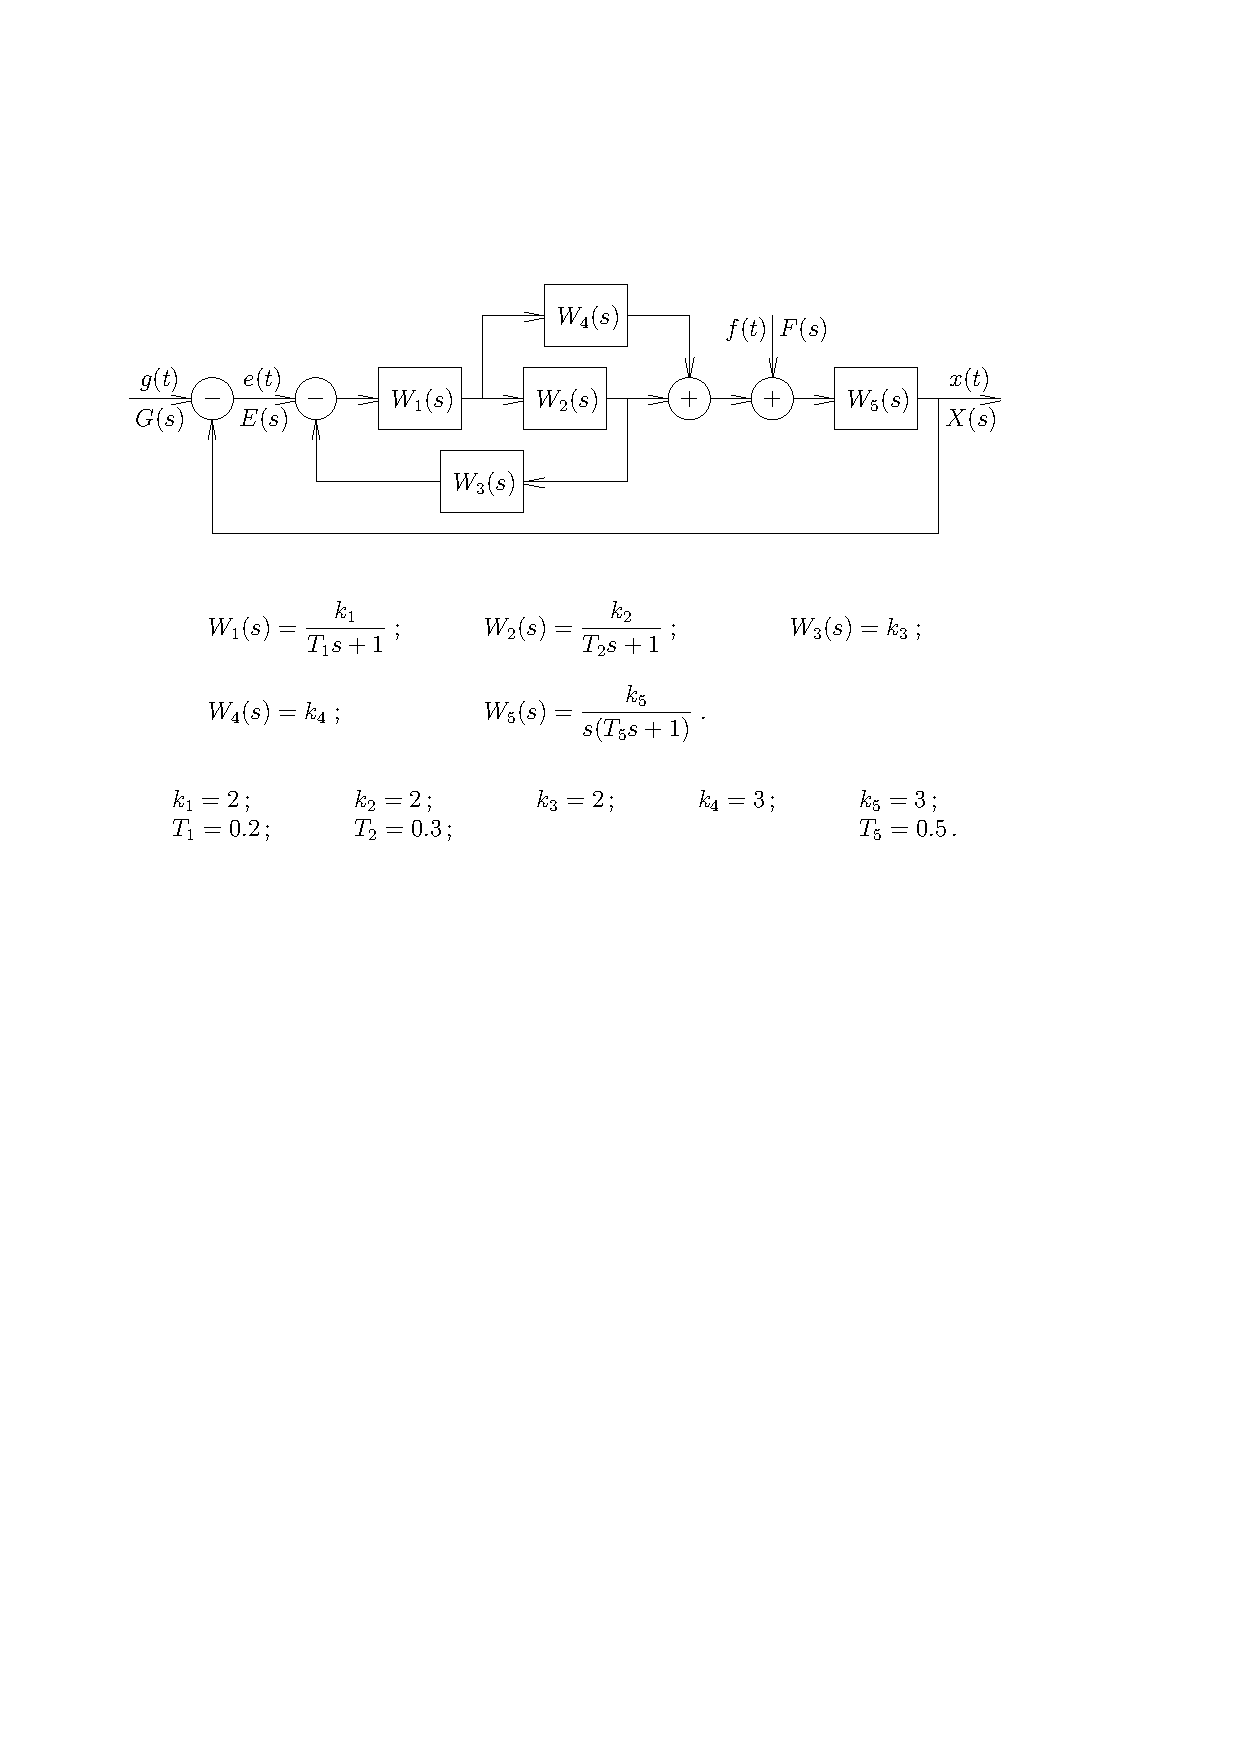
\includegraphics[scale=1,page=1]{Схема_1.pdf}
	\end{center}
	%$\\$
	
	\newpage
	
	\textbf{Задание 1.} Составить уравнения динамики разомкнутой и замкнутой систем в пространстве состояний (определить матрицу $A$, векторы $\overline{b}$, $\overline{c}^T$, коэффициент $d$).
	$\\$
	
	Для разомкнутой схемы:
	
	\begin{center}
		
\includegraphics[scale=1,page=1]{Схема_разомкн.png}
	\end{center}
	
	$\ds \mathrm{x}_1 = x$
	
	$\ds \mathrm{x}_2 = T_5 \frac{d \mathrm{x}_1}{dt} + \mathrm{x}_1$
	\vs
	
	$\ds \frac{1}{k_5} \frac{d \mathrm{x}_2}{dt} = \mathrm{x}_3 + k_4 \mathrm{x}_4 $
	\vs
	
	$\ds \mathrm{x}_4 = \frac{1}{k_2} \bigg( T_2 \frac{d \mathrm{x}_3}{dt} + \mathrm{x}_3 \bigg)$
	\vs
	
	$\ds \frac{1}{k_1} \bigg( T_1 \frac{d \mathrm{x}_4}{dt} + \mathrm{x}_4 \bigg) = g - k_3 \mathrm{x}_3$
	
	$\\$
	
%	Отсюда уравнение динамики разомкнутой системы:
	
	$\begin{cases}
		\ds \frac{d \mathrm{x}_1}{dt} = - \frac{1}{T_5} \mathrm{x}_1 + \frac{1}{T_5} \mathrm{x}_2 \\
		\ds \frac{d \mathrm{x}_2}{dt} = k_5 \mathrm{x}_3 + k_4 k_5 \mathrm{x}_4 \\
		\ds \frac{d \mathrm{x}_3}{dt} = - \frac{1}{T_2} \mathrm{x}_3 + \frac{k_2}{T_2} \mathrm{x}_4 \\
		\ds \frac{d \mathrm{x}_4}{dt} = - \frac{k_1 k_3}{T_1} \mathrm{x}_3 - \frac{1}{T_1} \mathrm{x}_4 + \frac{k_1}{T_1} g
	\end{cases}$
	\vs
	
	$\ds \mathrm{x}_1 = x$
	$\\$
	
	$\ds A = \begin{pmatrix}
		- \frac{1}{T_5} & \frac{1}{T_5} & 0 & 0 \\
		0 & 0 & k_5 & k_4 k_5 \\
		0 & 0 & - \frac{1}{T_2} & \frac{k_2}{T_2} \\
		0 & 0 & - \frac{k_1 k_3}{T_1} & - \frac{1}{T_1}
	\end{pmatrix}$\hspace{1.0cm}
	$\ds \overline{b} = \begin{pmatrix}
		0 \\
		0 \\
		0 \\
		\frac{k_1}{T_1}
	\end{pmatrix}$\hspace{1.0cm}
	$\ds \overline{c}^T = \begin{pmatrix} 1 & 0 & 0 & 0 \end{pmatrix}$\hspace{1.0cm}
	$\ds d = 0$
	
	$\\$
	
	$\ds A = \begin{pmatrix}
		- 2 & 2 & 0 & 0 \\
		0 & 0 & 3 & 9 \\
		0 & 0 & - 3.33 & 6.67 \\
		0 & 0 & - 20 & - 5
	\end{pmatrix}$\hspace{1.0cm}
	$\ds \overline{b} = \begin{pmatrix}
		0 \\
		0 \\
		0 \\
		10
	\end{pmatrix}$\hspace{1.0cm}
	$\ds \overline{c}^T = \begin{pmatrix} 1 & 0 & 0 & 0 \end{pmatrix}$\hspace{1.0cm}
	$\ds d = 0$
	%$\\$
	\newpage
	
	
	Для замкнутой схемы:
	
	\begin{center}
		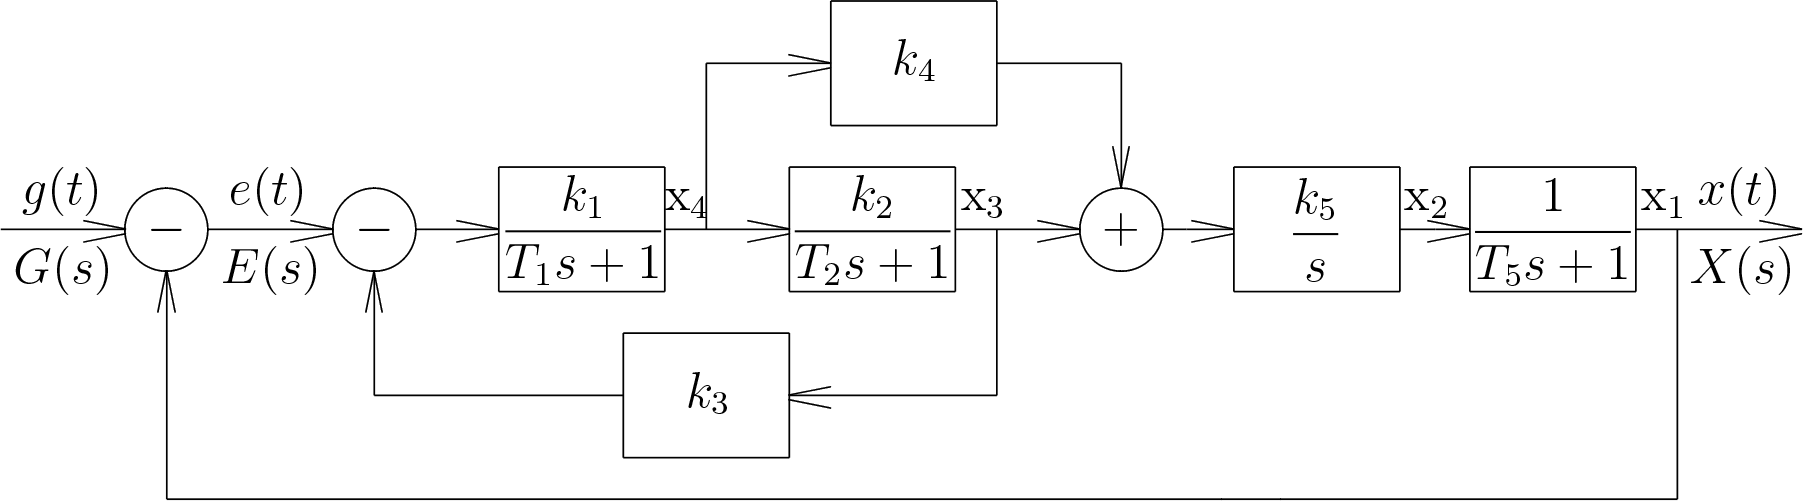
\includegraphics[scale=1,page=1]{Схема_замкн.png}
	\end{center}
	
	$\ds \mathrm{x}_1 = x$
	
	$\ds \mathrm{x}_2 = T_5 \frac{d \mathrm{x}_1}{dt} + \mathrm{x}_1$
	\vs
	
	$\ds \frac{1}{k_5} \frac{d \mathrm{x}_2}{dt} = \mathrm{x}_3 + k_4 \mathrm{x}_4 $
	\vs
	
	$\ds \mathrm{x}_4 = \frac{1}{k_2} \bigg( T_2 \frac{d \mathrm{x}_3}{dt} + \mathrm{x}_3 \bigg)$
	\vs
	
	$\ds \frac{1}{k_1} \bigg( T_1 \frac{d \mathrm{x}_4}{dt} + \mathrm{x}_4 \bigg) = g - \mathrm{x}_1 - k_3 \mathrm{x}_3$
	
	$\\$
	
	$\begin{cases}
		\ds \frac{d \mathrm{x}_1}{dt} = - \frac{1}{T_5} \mathrm{x}_1 + \frac{1}{T_5} \mathrm{x}_2 \\
		\ds \frac{d \mathrm{x}_2}{dt} = k_5 \mathrm{x}_3 + k_4 k_5 \mathrm{x}_4 \\
		\ds \frac{d \mathrm{x}_3}{dt} = - \frac{1}{T_2} \mathrm{x}_3 + \frac{k_2}{T_2} \mathrm{x}_4 \\
		\ds \frac{d \mathrm{x}_4}{dt} = - \frac{k_1}{T_1} \mathrm{x}_1 - \frac{k_1 k_3}{T_1} \mathrm{x}_3 - \frac{1}{T_1} \mathrm{x}_4 + \frac{k_1}{T_1} g
	\end{cases}$
	\vs
	
	$\ds \mathrm{x}_1 = x$
	$\\$
	
	$\ds A = \begin{pmatrix}
		- \frac{1}{T_5} & \frac{1}{T_5} & 0 & 0 \\
		0 & 0 & k_5 & k_4 k_5 \\
		0 & 0 & - \frac{1}{T_2} & \frac{k_2}{T_2} \\
		- \frac{k_1}{T_1} & 0 & - \frac{k_1 k_3}{T_1} & - \frac{1}{T_1}
	\end{pmatrix}$\hspace{1.0cm}
	$\ds \overline{b} = \begin{pmatrix}
		0 \\
		0 \\
		0 \\
		\frac{k_1}{T_1}
	\end{pmatrix}$\hspace{1.0cm}
	$\ds \overline{c}^T = \begin{pmatrix} 1 & 0 & 0 & 0 \end{pmatrix}$\hspace{1.0cm}
	$\ds d = 0$
	
	$\\$
	
	$\ds A = \begin{pmatrix}
		- 2 & 2 & 0 & 0 \\
		0 & 0 & 3 & 9 \\
		0 & 0 & - 3.33 & 6.67 \\
		-10 & 0 & - 20 & - 5
	\end{pmatrix}$\hspace{1.0cm}
	$\ds \overline{b} = \begin{pmatrix}
		0 \\
		0 \\
		0 \\
		10
	\end{pmatrix}$\hspace{1.0cm}
	$\ds \overline{c}^T = \begin{pmatrix} 1 & 0 & 0 & 0 \end{pmatrix}$\hspace{1.0cm}
	$\ds d = 0$
	
	
	\newpage
	
	\textbf{Задание 2.} Определить передаточную функцию разомкнутой системы $W(s)$, приведя ее к типовым звеньям. Построить ЛАФЧХ разомкнутой системы на ЛАХ-бумаге. Определить передаточную функцию замкнутой системы $\Phi(s)$.
	$\\$
	
	Разомкнутая система:
	
	\begin{center}
		
\includegraphics[scale=1,page=1]{Схема_разомкн_2.png}
	\end{center}
	%$\\$

	
\includegraphics[scale=0.8,page=1]{Схема_преобр_1.png}
	$\\$

	
\includegraphics[scale=0.8,page=1]{Схема_преобр_2.png}
	$\\$
	
	
\includegraphics[scale=0.8,page=1]{Схема_преобр_3.png}
	$\\$
	
	
\includegraphics[scale=0.8,page=1]{Схема_преобр_4.png}
	$\\$
	
	
\includegraphics[scale=0.8,page=1]{Схема_преобр_5.png}
	$\\$
	
	
\includegraphics[scale=0.8,page=1]{Схема_преобр_6.png}
	%$\\$
	\newpage

	$\ds W(s) = \frac{W_1(s) W_5(s) \big( W_2(s) + W_4(s) \big)}{1 + W_1(s) W_2(s) W_3(s)} = \frac{\frac{k_1}{T_1 s + 1} \cdot \frac{k_5}{s (T_5 s + 1)} \cdot \left( \frac{k_2}{T_2 s + 1} + k_4 \right)}{1 + \frac{k_1}{T_1 s + 1} \cdot \frac{k_2}{T_2 s + 1} \cdot k_4} = $
	\vs
	
	$\ds = \frac{k_1 k_5 (k_2 + k_4 + k_4 T_2 s)}{s (T_1 s + 1) (T_5 s + 1) (T_2 s + 1)} \; \frac{(T_1 s + 1) (T_2 s + 1)}{(T_1 s + 1) (T_2 s + 1) + k_1 k_2 k_3} = $
	\vs
	
	$\ds = \frac{k_1 k_5 (k_2 + k_4 + k_4 T_2 s)}{s (T_5 s + 1) \big(T_1 T_2 s^2 + (T_1 + T_2) s + 1 + k_1 k_2 k_3\big)} = $
	\vs
	
	$\ds = \frac{k_1 k_5 (k_2 + k_4)}{1 + k_1 k_2 k_3} \bigg(1 + \frac{k_4 T_2}{k_2 + k_4} s \bigg) \frac{1}{s} \; \frac{1}{T_5 s + 1} \; \frac{1}{\frac{T_1 T_2}{1 + k_1 k_2 k_3} s^2 + \frac{T_1 + T_2}{1 + k_1 k_2 k_3} s + 1} = $
	\vs
	
	$\ds = \frac{10}{3} \; (1 + 0.18 s) \; \frac{1}{s} \; \frac{1}{0.5 s + 1} \; \frac{1}{\frac{2}{300} s^2 + \frac{5}{90} s + 1}$
	$\\$
	
	ЛАФЧХ разомкнутой системы (вместе с асимптотическими графиками):
	
	\begin{center}
		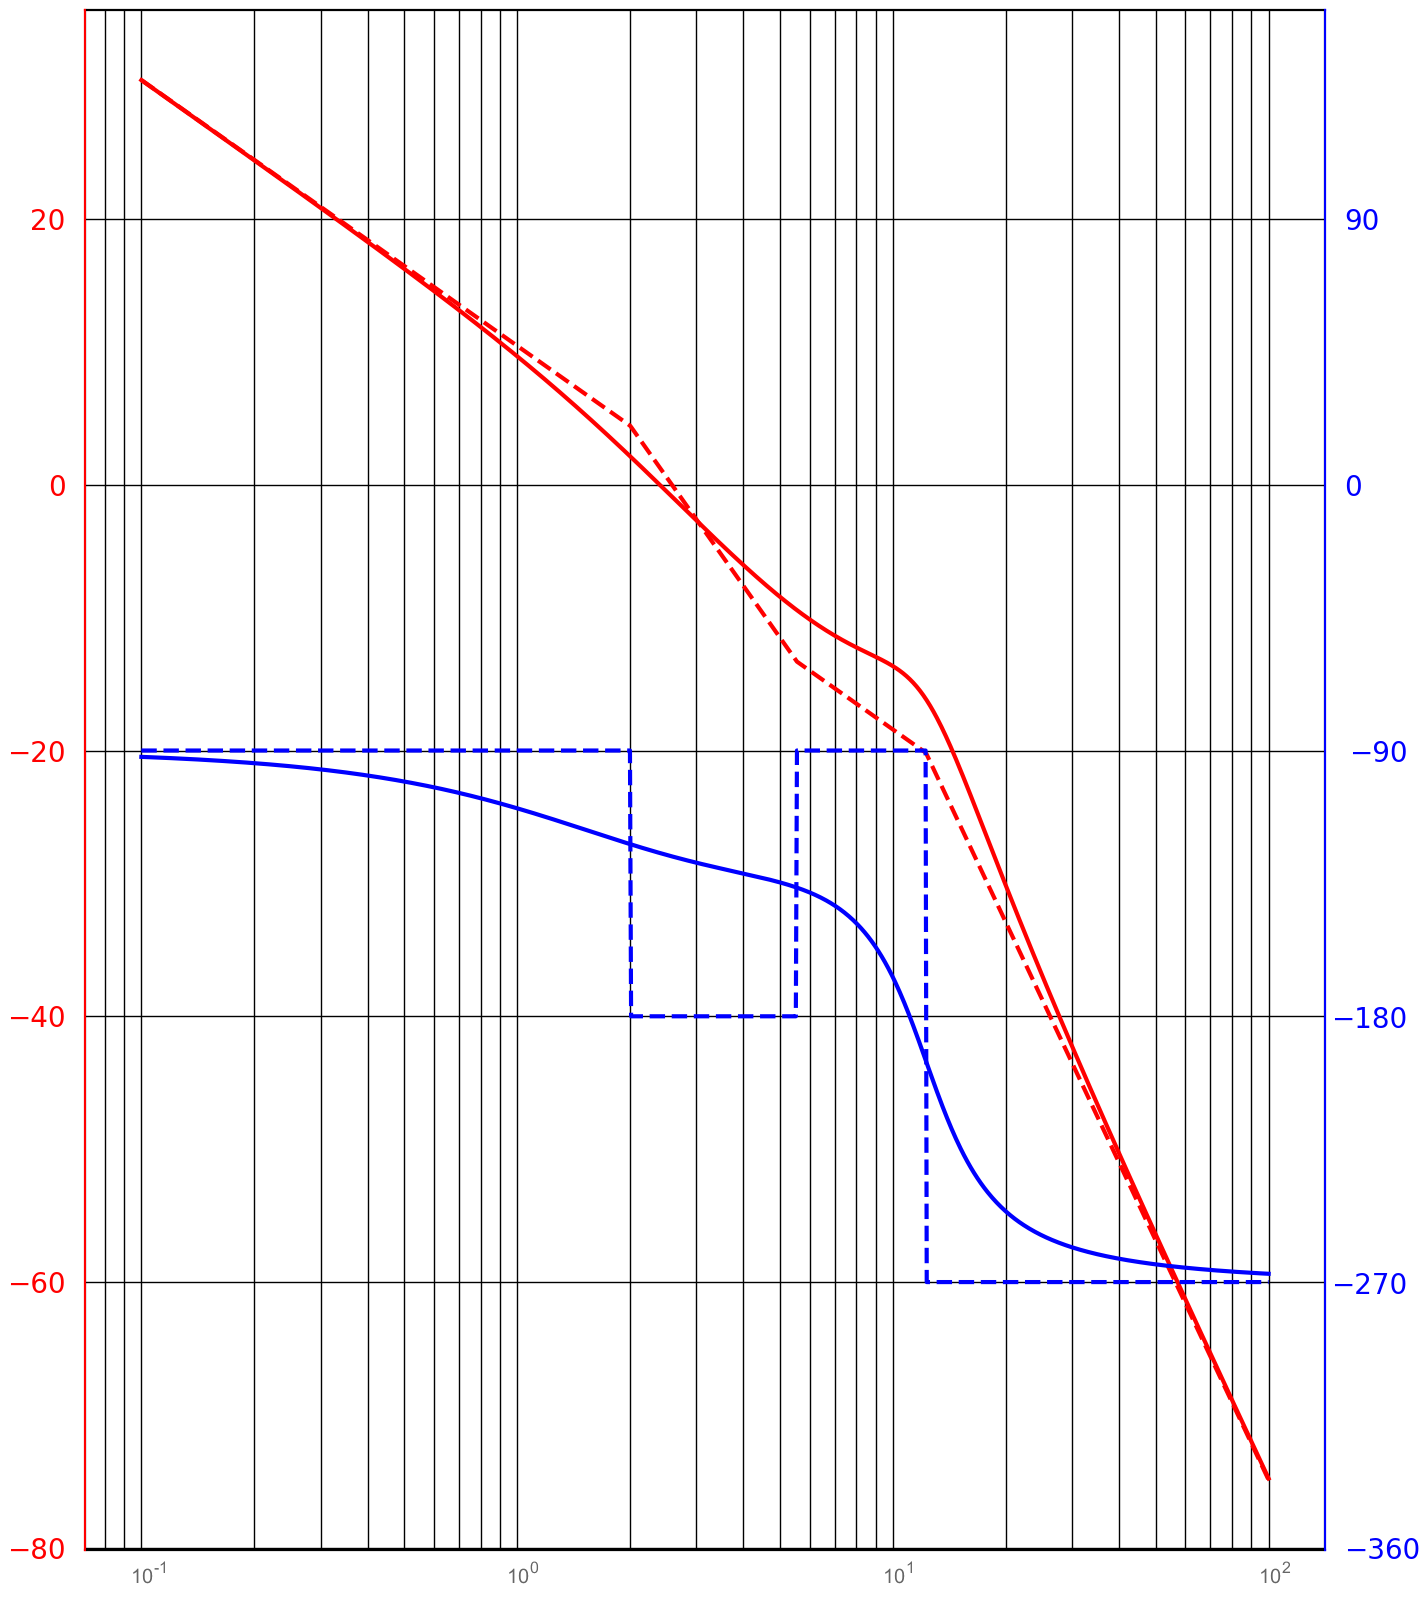
\includegraphics[scale=0.85,page=1]{ЛАФЧХ.png}
	\end{center}
	
	Замкнутая система:
	
	\begin{center}
		
\includegraphics[scale=1,page=1]{Схема_преобр_7.png}
	\end{center}
	
	$\ds \Phi(s) = \frac{W(s)}{1 + W(s)} = \frac{\frac{10}{3} \; (1 + 0.18 s) \; \frac{1}{s} \; \frac{1}{0.5 s + 1} \; \frac{1}{\frac{2}{300} s^2 + \frac{5}{90} s + 1}}{1 + \frac{10}{3} \; (1 + 0.18 s) \; \frac{1}{s} \; \frac{1}{0.5 s + 1} \; \frac{1}{\frac{2}{300} s^2 + \frac{5}{90} s + 1}} = $
	\vs
	
	$\ds = \frac{10}{3} \; (1 + 0.18 s) \; \frac{1}{s (0.5 s + 1) \left( \frac{2}{300} s^2 + \frac{5}{90} s + 1 \right) + \frac{10}{3} (0.18 s + 1)} = $
	\vs
	
	$\ds = (1 + 0.18 s) \; \frac{1}{0.001 s^4 + \frac{31}{300} s^3 + \frac{1}{6} s^2 + 0.48 s + 1}$
	
	\newpage
	
	\textbf{Задание 3.} Построить на компьютере АФЧХ (годограф) и ЛАФЧХ разомкнутой и замкнутой систем.
	$\\$
	
	ЛАФЧХ разомкнутой системы:
	
	\hspace{-3.0cm}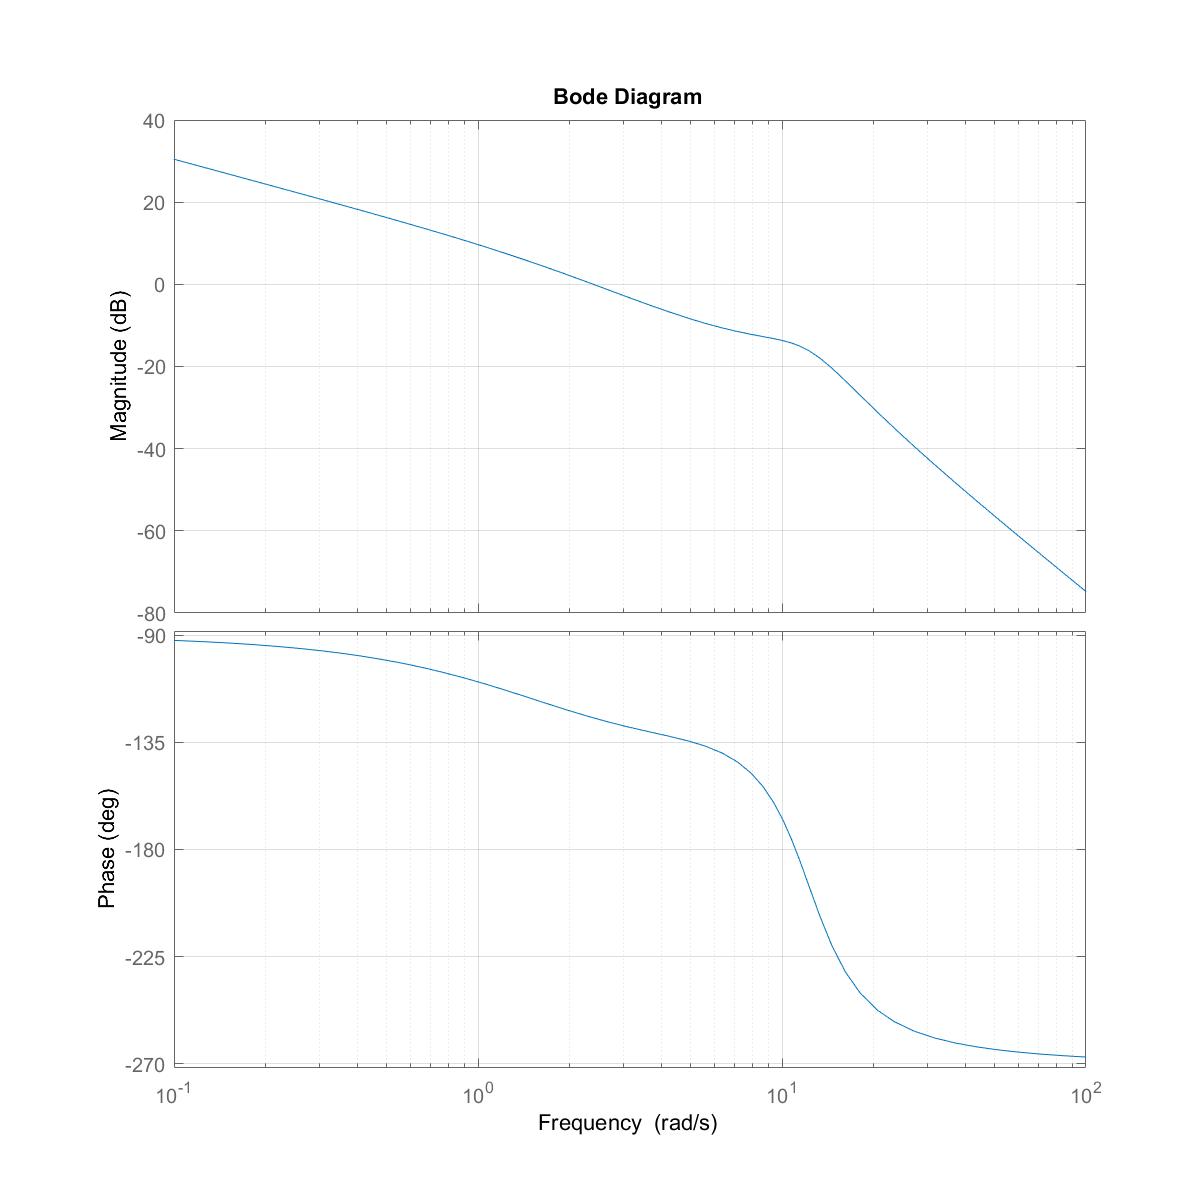
\includegraphics[scale=0.65,page=1]{ЛАФЧХ_3(1.1).png}
	
	\newpage
	
	ЛАФЧХ замкнутой системы:
	
	\hspace{-3.0cm}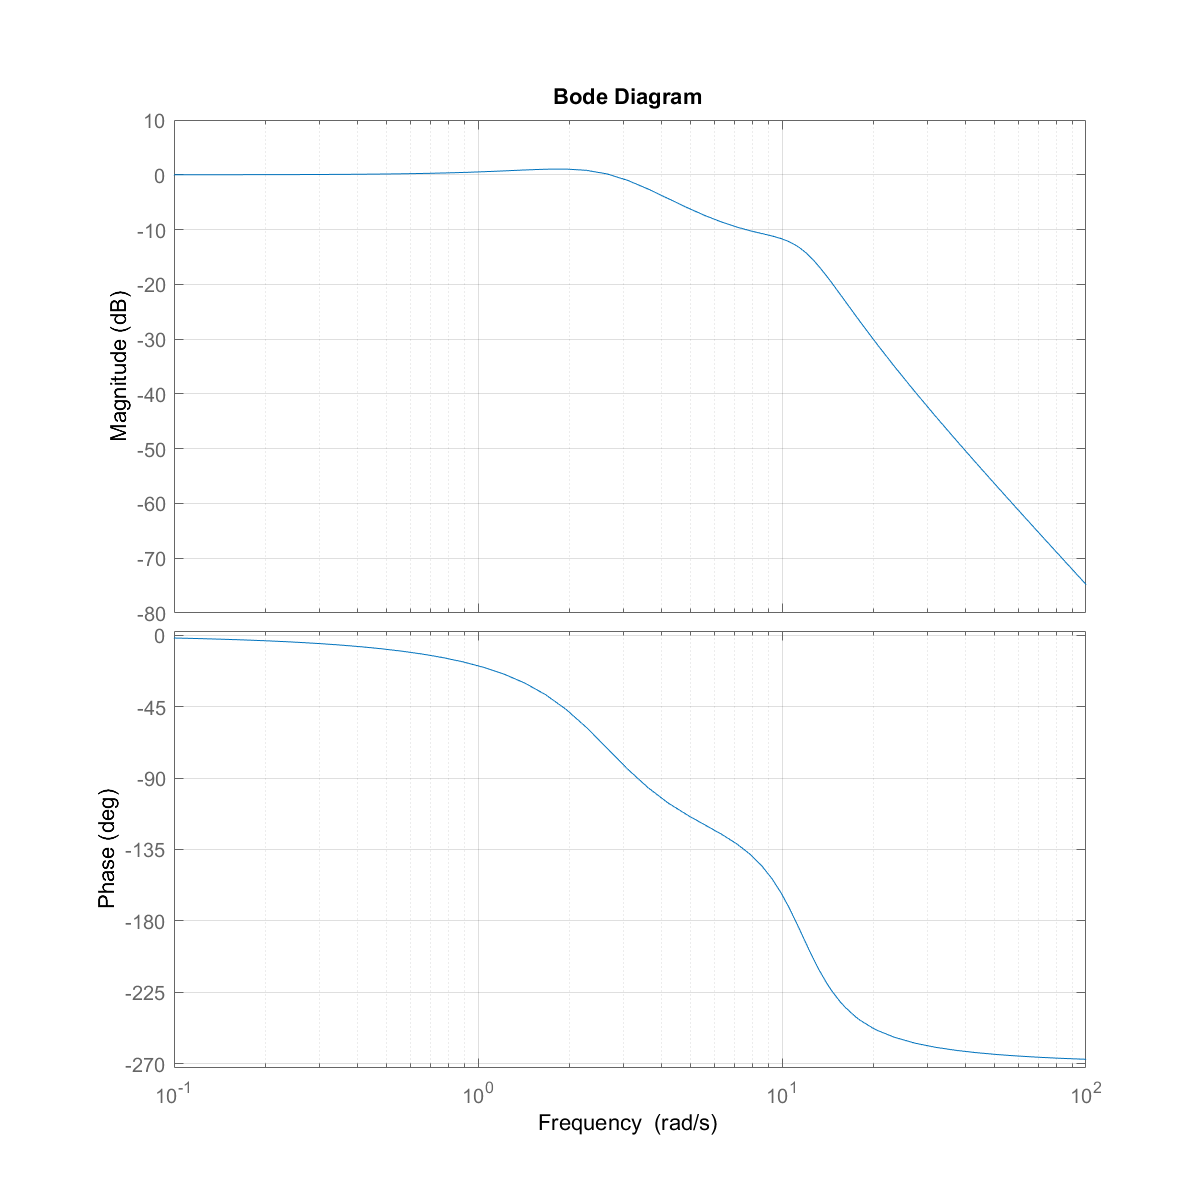
\includegraphics[scale=0.65,page=1]{ЛАФЧХ_3(2.1).png}
	
	\newpage
	
	АФЧХ (годограф) разомкнутой системы:
	
	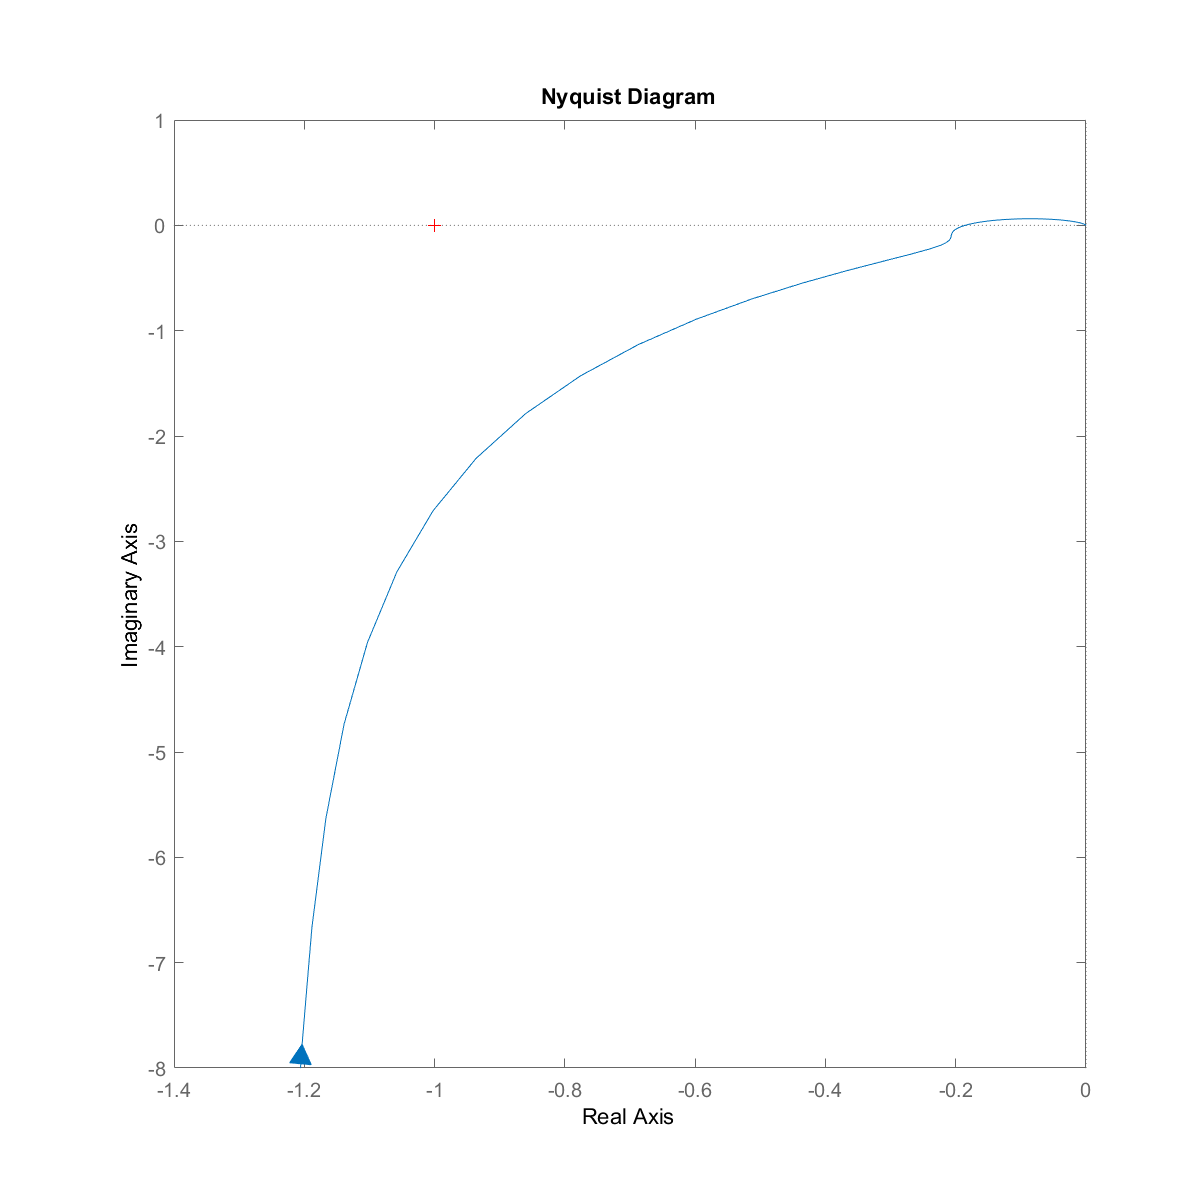
\includegraphics[scale=0.38,page=1]{АФЧХ_3(1.1).png}
	
	АФЧХ (годограф) замкнутой системы:
	
	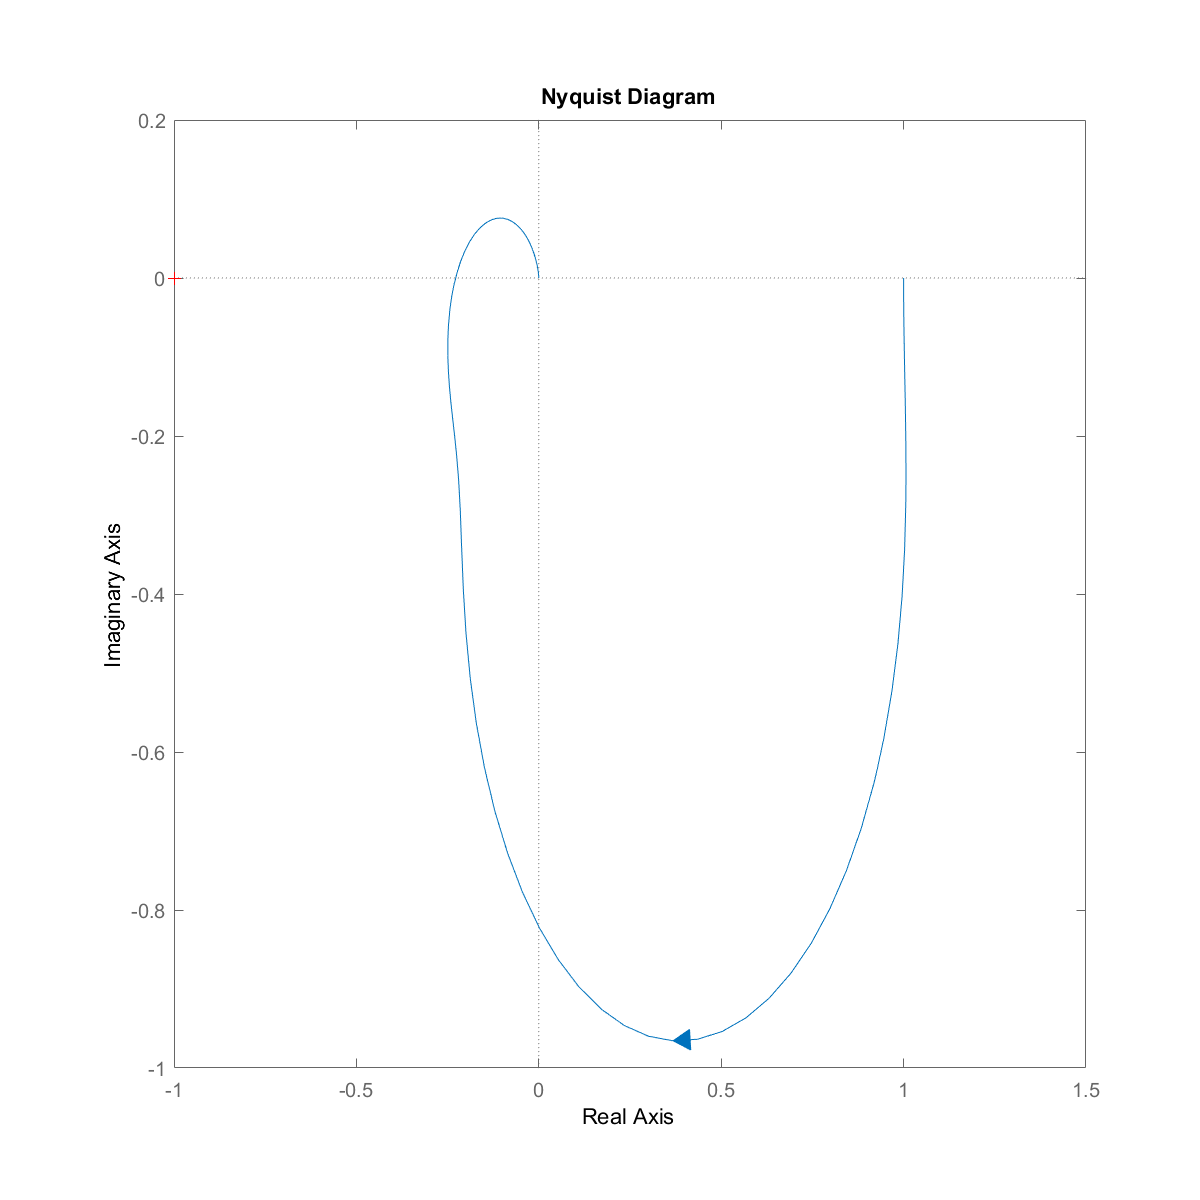
\includegraphics[scale=0.38,page=1]{АФЧХ_3(2.1).png}
	
	
	\newpage
	
	\textbf{Задание 4.} Исследовать устойчивость системы с использованием ЛАФЧХ и частотного критерия. Определить предельный коэффициент усиления системы, при котором система находится на грани устойчивости.
	$\\$
	
	По критерию Найквиста: для устойчивости замкнутой ЛДС необходимо и достаточно, чтобы её годограф в разомкнутом состоянии охватывал критическую точку $(-1; 0 j)$ против часовой стрелки $K/2$ раз при возрастании частоты $0 \leqslant \omega < +\infty$, где $K$ -- число полюсов передаточной функции разомкнутой системы в правой полуплоскости.
	$\\$
	
	Передаточная функция разомкнутой системы:
	\vs
	
	$\ds W(s) = \frac{10}{3} \; (1 + 0.18 s) \; \frac{1}{s} \; \frac{1}{0.5 s + 1} \; \frac{1}{\frac{2}{300} s^2 + \frac{5}{90} s + 1}$
	\vs
	
	Полюсы $W(s)$: \; $\ds \l_1 = 0$, \, $\ds \l_2 = - 2$, \, $\ds \l_{3,4} \approx - 4.1667 \pm 11.5169 j$. Ни один из полюсов не расположен в правой полуплоскости, так что $K = 0$.
	
	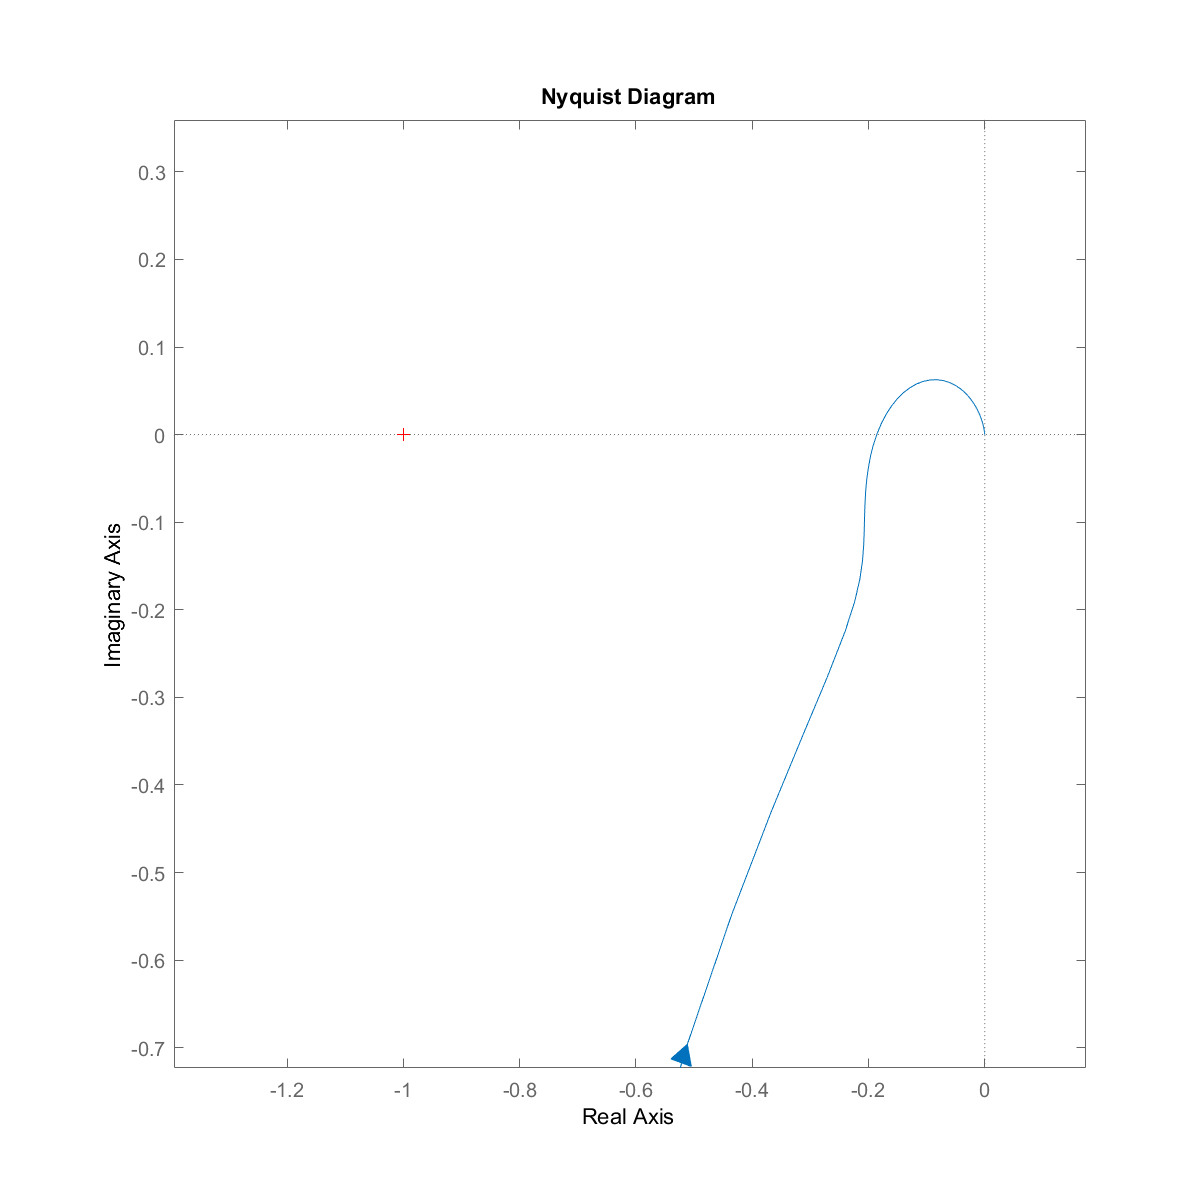
\includegraphics[scale=0.38,page=1]{АФЧХ_3(1.2).png}
	
	Из построенного рисунка видно, что годограф не охватывает точку $(-1,0 j)$ (т. е. охватывает её 0 раз). Поэтому выполняется равенство:
	
	$\ds 0 = \frac{0}{2}$ -- то есть система устойчива.
	
	
	Сделаем коэффициент усиления звеньев $\ds k = \frac{10}{3}$ варьируемой переменной:
	\vs
	
	$\ds W(s) = k \; (1 + 0.18 s) \; \frac{1}{s} \; \frac{1}{0.5 s + 1} \; \frac{1}{\frac{2}{300} s^2 + \frac{5}{90} s + 1}$
	$\\$
	
	Тогда ЛАЧХ данной передаточной функции будет совершать вертикальный параллельный перенос при изменении значения k.
	
	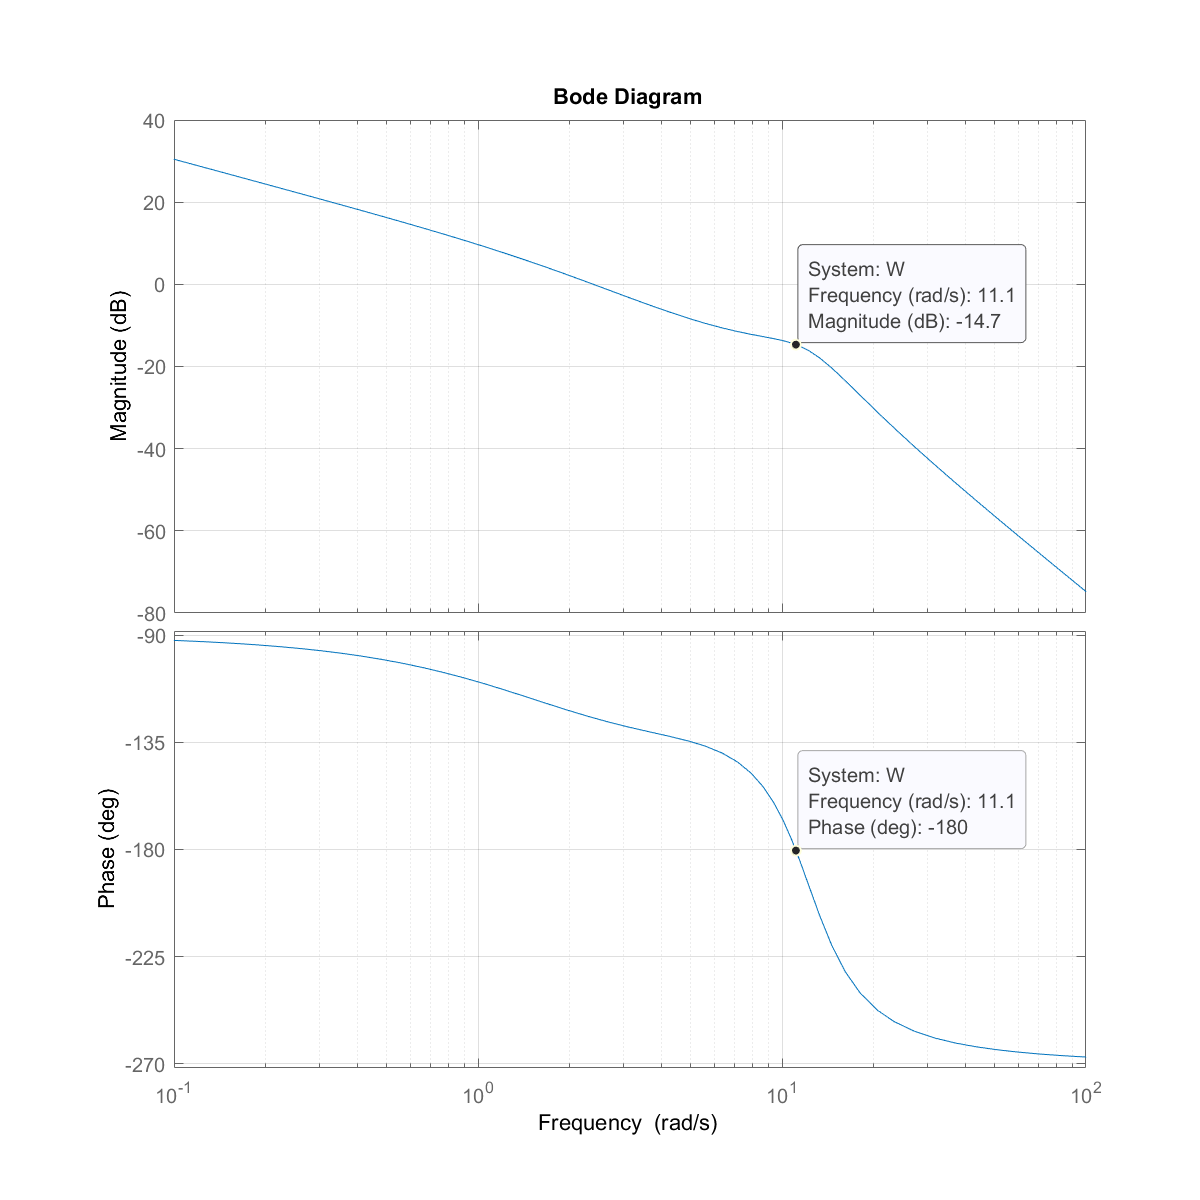
\includegraphics[scale=0.5,page=1]{ЛАФЧХ_3(1.2).png}
	
	Из рисунка видно, что запас устойчивости по амплитуде $h_m \approx 14.7$ -- на такую величину можно параллельно переносить ЛАЧХ вверх, прежде чем её точка пересечения с нулём окажется правее, чем точка пересечения ФЧХ со значением $-180$, в случае чего система уже окажется неустойчивой.
	
	Тогда:
	
	$\ds 20 \lg k_{\text{кр}} = 20 \lg \frac{10}{3} + h_m$
	
	$\ds k_{\text{кр}} = \frac{10}{3} \cdot 10^{h_m/20} \approx 18$ -- при таком $k$ система находится на грани устойчивости.
	
	\hspace{-2.0cm}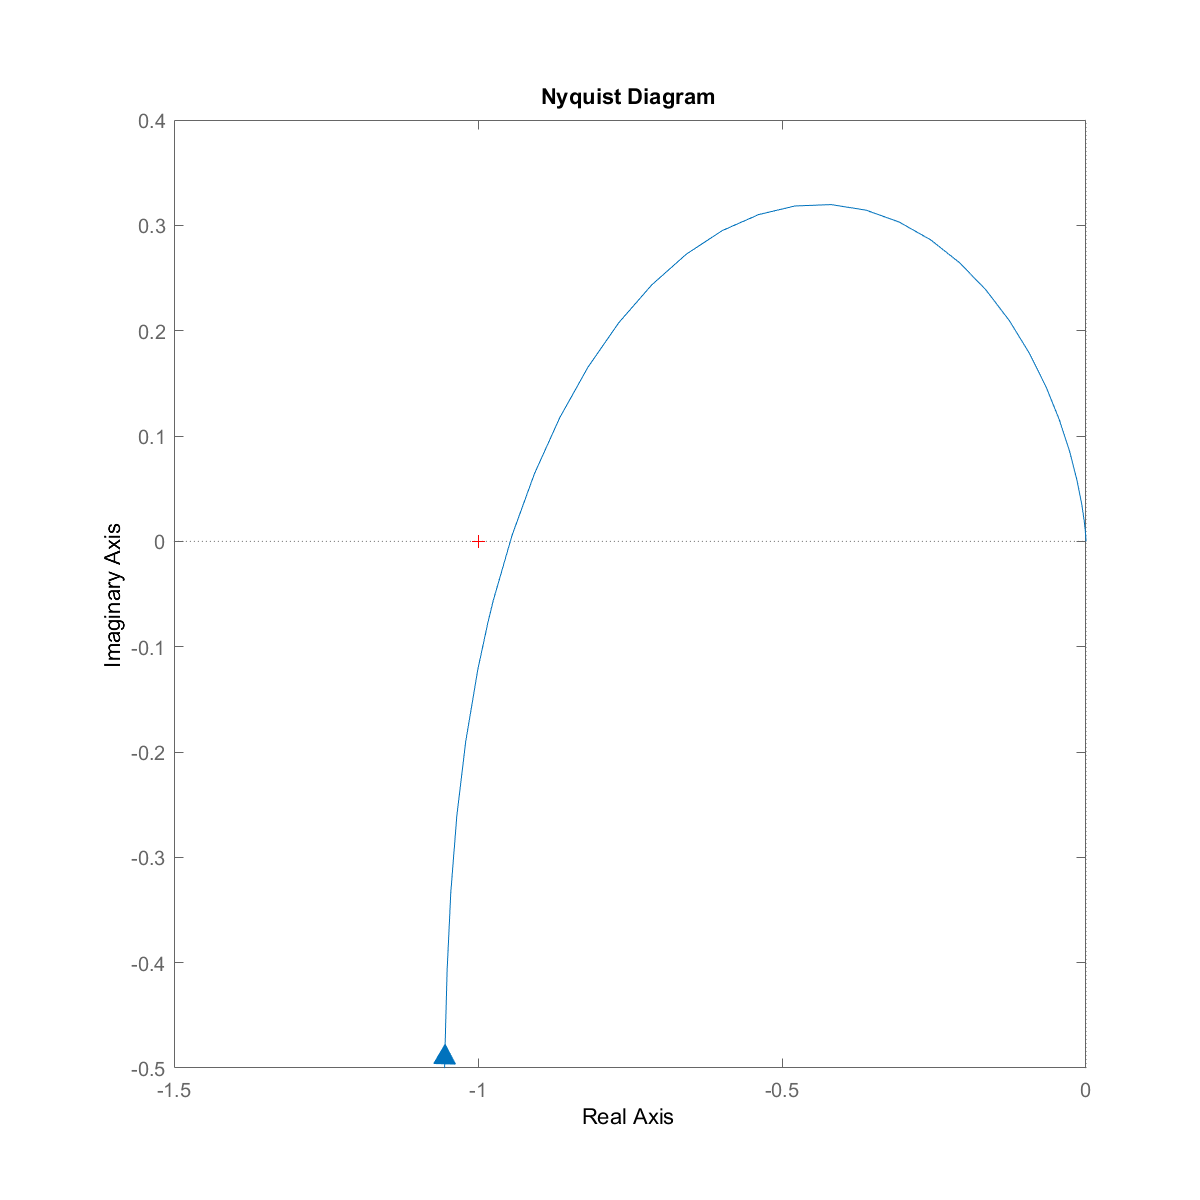
\includegraphics[scale=0.30,page=1]{АФЧХ_3(1.k17).png}
	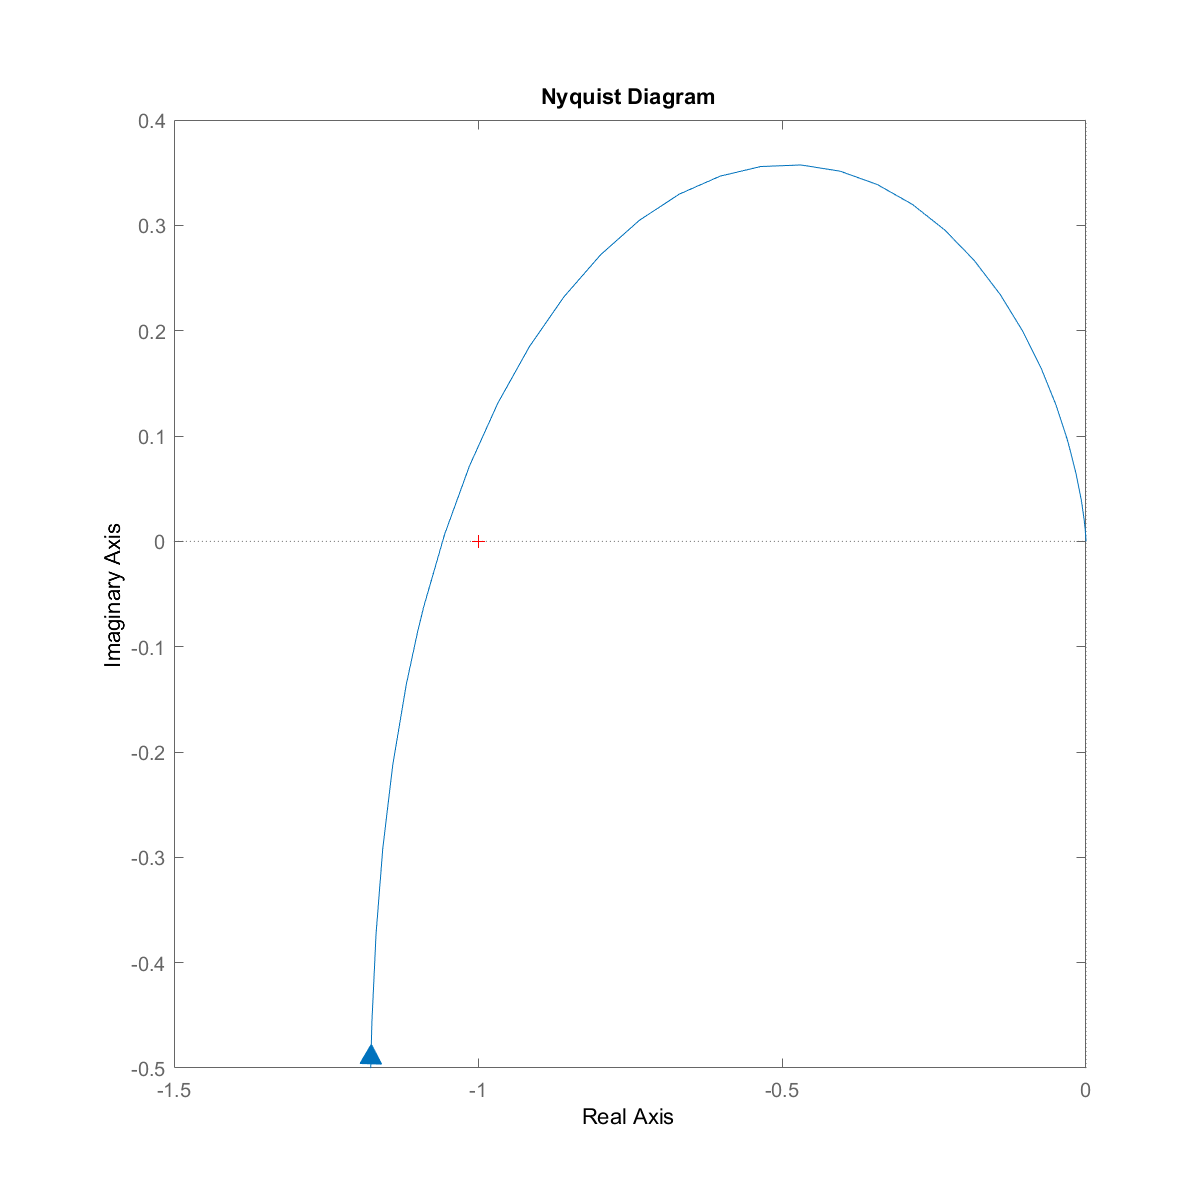
\includegraphics[scale=0.30,page=1]{АФЧХ_3(1.k19).png}
	
	Выше приведены АФЧХ для случаев $k = 17$ и $k = 19$ соответственно. Видно, что в первом случае годограф не охватывает точку $(-1,0 j)$ (т. е. охватывает её 0 раз), поэтому выполняется равенство $\ds 0 = \frac{0}{2}$, и система оказывается устойчивой. А во втором случае годограф охватывает точку $(-1,0 j)$ 1 раз по часовой стрелке (т. е. охватывает $-1$ раз против часовой стрелки), поэтому выражение $\ds -1 = \frac{0}{2}$ не является равенством, и система оказывается неустойчивой.
	
	
	\newpage
	
	\textbf{Задание 5.} Построить на компьютере переходные процессы в замкнутой системе при действии единичного ступенчатого, линейного нарастающего и гармонического воздействий. Определить астатизм, коэффициенты добротности системы и предельные значения установившихся ошибок при $g(t) = 1 [t]$, $g(t) = at$. Определить коэффициенты ошибок $C_0$, $C_1$, $C_2$.
	$\\$
	
	Для построения переходных процессов при заданных воздействиях использовалась команда \texttt{lsim(sys,g,t)} в среде MATLAB.
	$\\$
	
	Переходный процесс при действии единичного ступенчатого воздействия:
	
	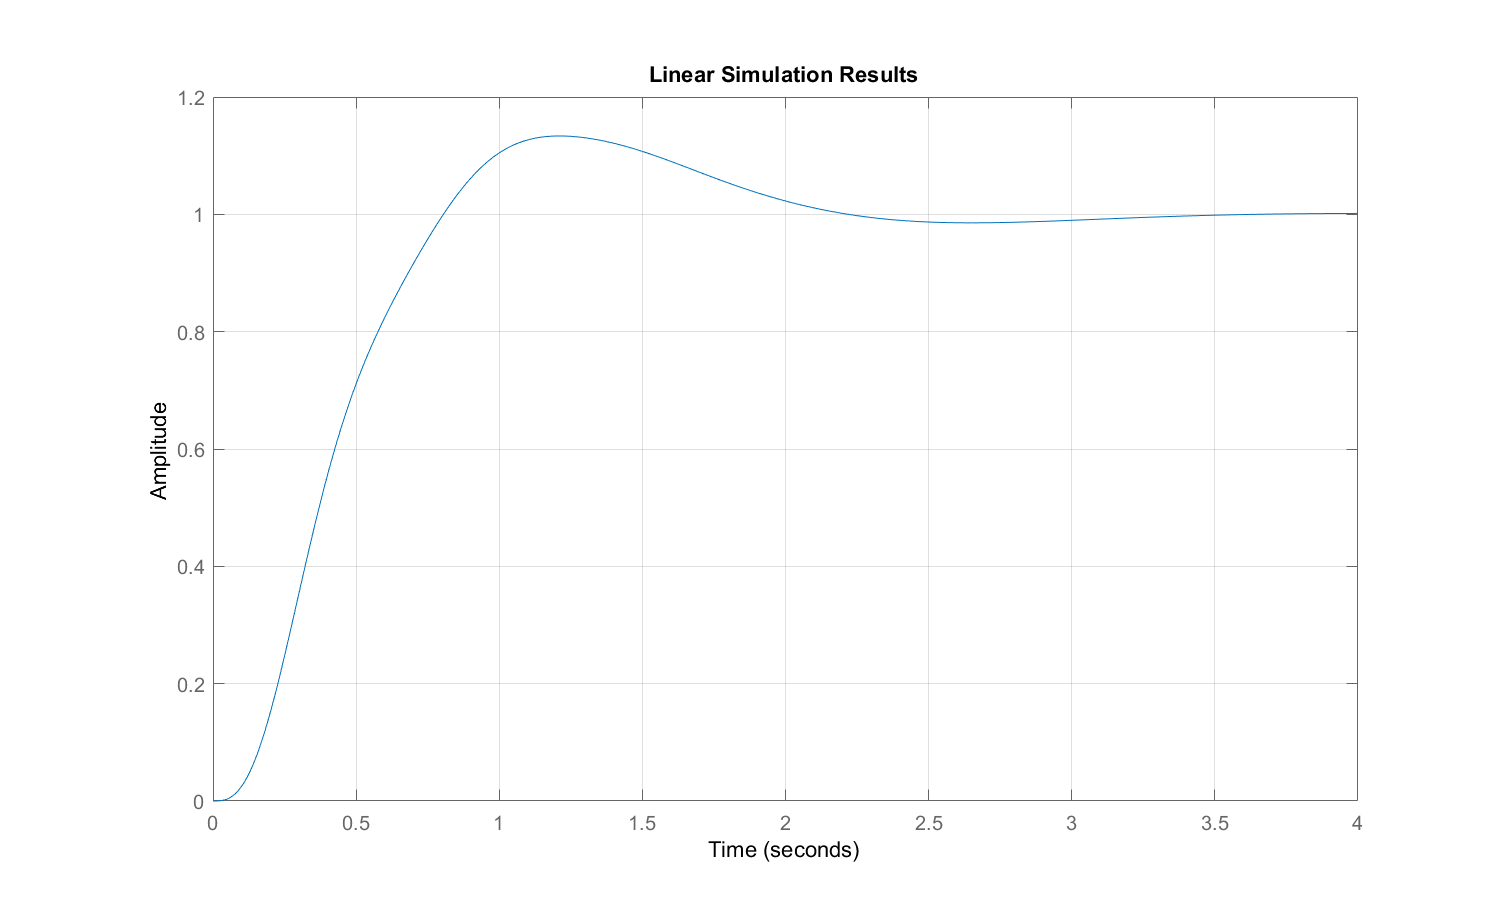
\includegraphics[scale=0.35,page=1]{ПП_1.png}
	\vs
	
	Переходный процесс при действии линейного нарастающего воздействия:
	
	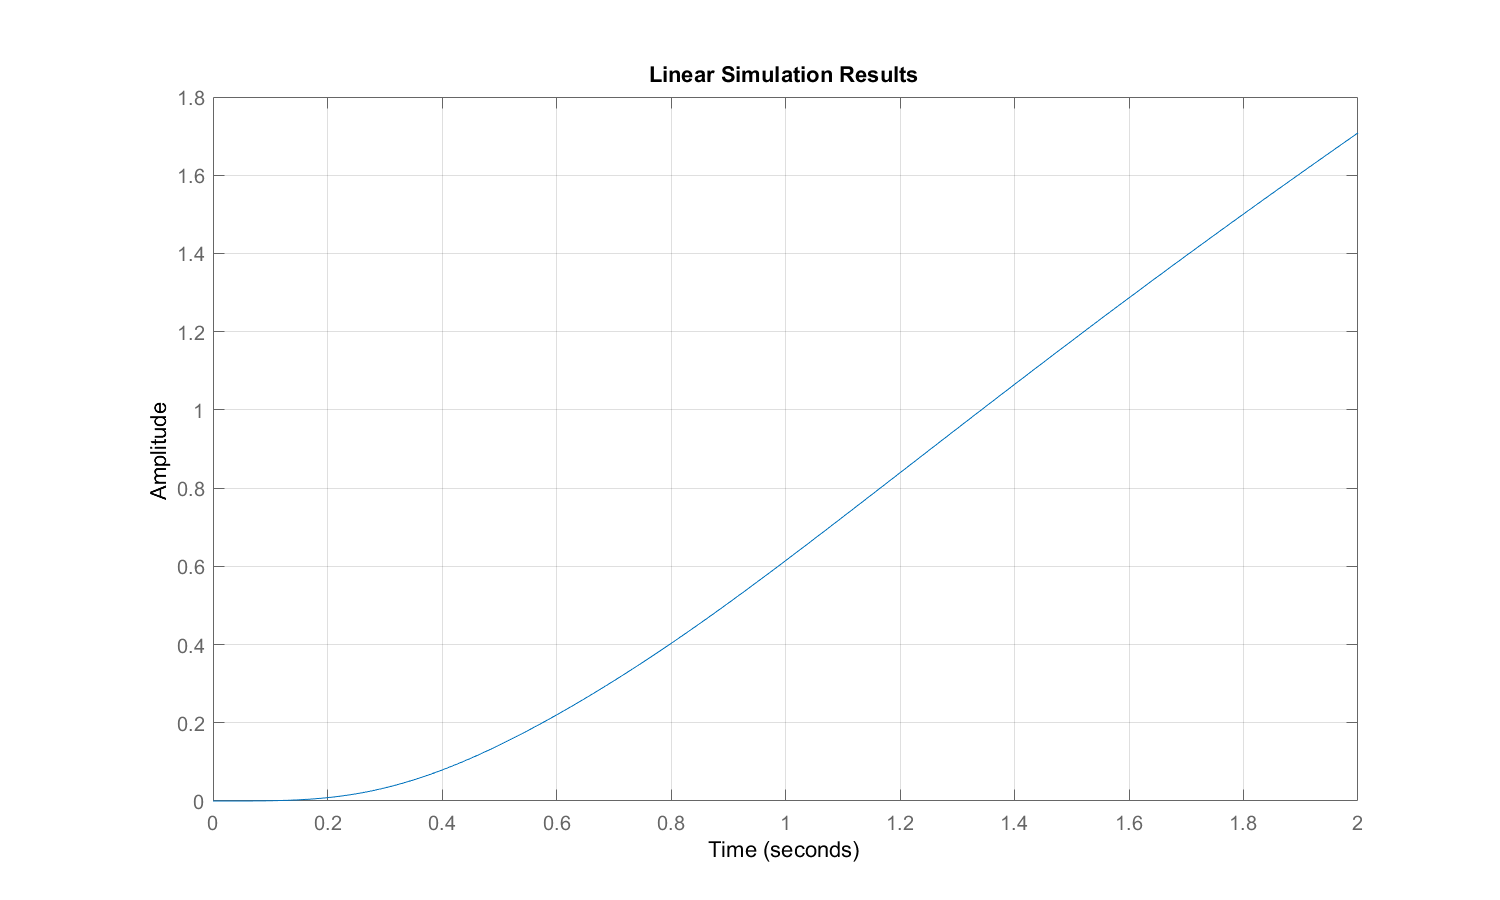
\includegraphics[scale=0.35,page=1]{ПП_2.png}
	
	Переходный процесс при действии гармонического воздействия:
	
	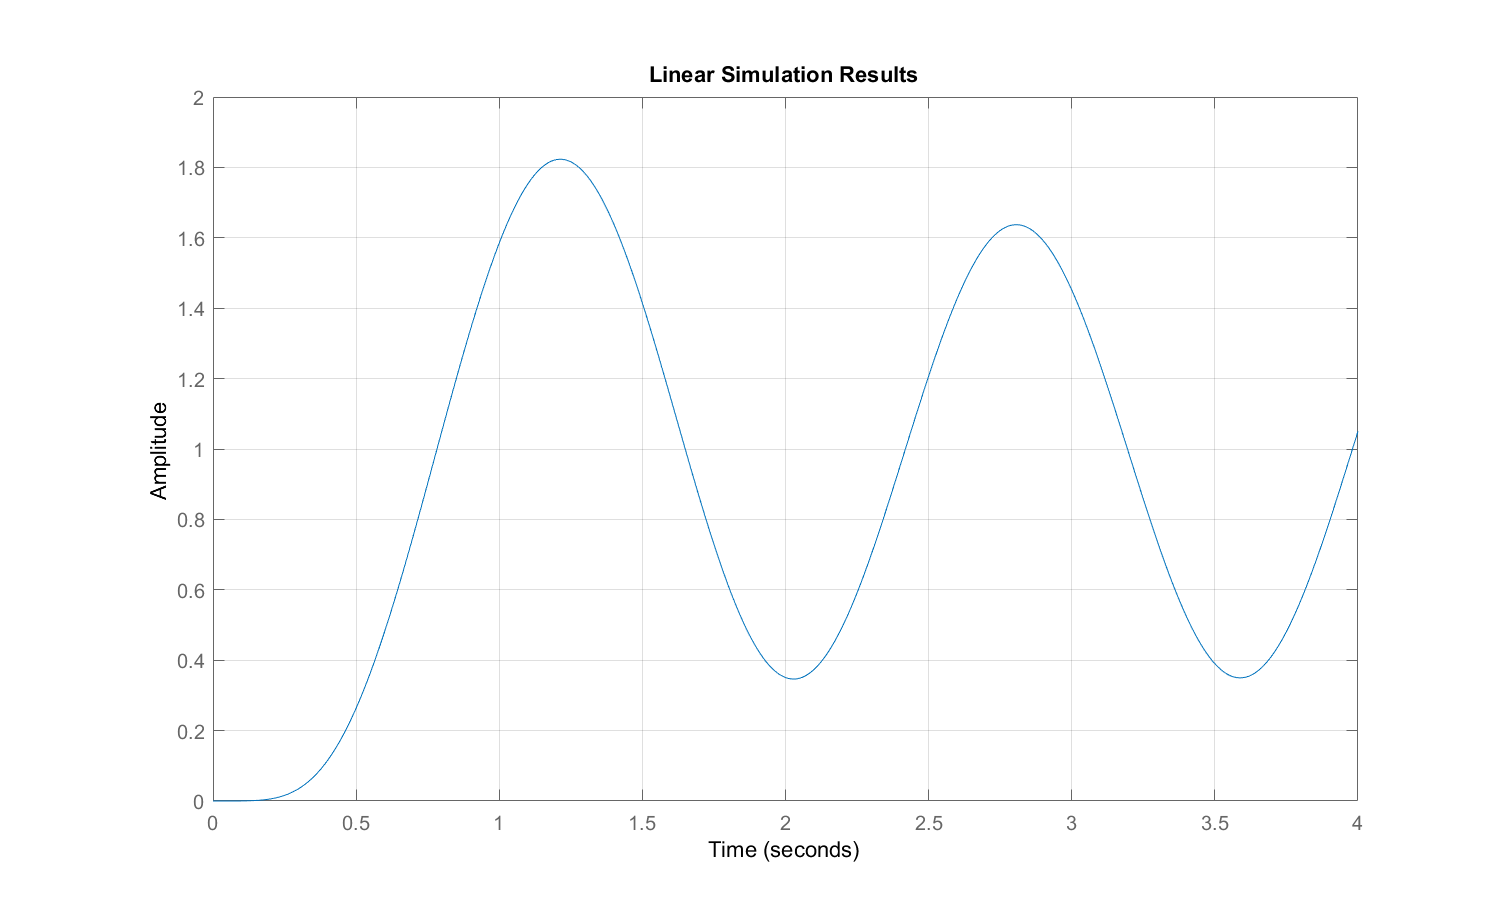
\includegraphics[scale=0.35,page=1]{ПП_3(2).png}
	$\\$
	
	Передаточная функция разомкнутой системы:
	\vs
	
	$\ds W(s) = \frac{10}{3} \; (1 + 0.18 s) \; \frac{1}{s} \; \frac{1}{0.5 s + 1} \; \frac{1}{\frac{2}{300} s^2 + \frac{5}{90} s + 1}$
	\vs
	
	В системе имеется одно интегрирующее звено, значит, система имеет \textbf{астатизм первого порядка}.
	
	$\nu = 1$
	$\\$
	
	%Коэффициент добротности по положению $\ds k_p = 1 + k = \frac{13}{3}$.
	
	Коэффициент добротности по скорости $\ds k_v = k = \frac{10}{3}$.
	%
	%Коэффициент добротности по ускорению $\ds k_a = k = \frac{10}{3}$.
	$\\$
	
	Передаточная функция замкнутой системы относительно ошибки $\e(t)$:
	\vs
	
	$\ds \Phi_\e(s) = \frac{1}{1 + W(s)} = \frac{1}{1 + \frac{10}{3} \; (0.18 s + 1) \; \frac{1}{s} \; \frac{1}{0.5 s + 1} \; \frac{1}{\frac{2}{300} s^2 + \frac{5}{90} s + 1}} = $
	\vs
	
	$\ds = \frac{s (0.5 s + 1) \left( \frac{2}{300} s^2 + \frac{5}{90} s + 1 \right)}{s (0.5 s + 1) \left( \frac{2}{300} s^2 + \frac{5}{90} s + 1 \right) + \frac{10}{3} (0.18 s + 1)} = $
	\vs
	
	$\ds = \frac{3}{10} s (1 + 0.5 s) \left( 1 + \frac{5}{90} s + \frac{2}{300} s^2 \right) \frac{1}{0.001 s^4 + \frac{31}{300} s^3 + \frac{1}{6} s^2 + 0.48 s + 1}$
	$\\$
	
	Коэффициенты ошибок:
	
	$\ds C_0 = \Phi_\e(0) = 0 $
	
	$\ds C_1 = \frac{d \Phi_\e}{ds} \bigg|_{s=0} = 0.3 $
	
	$\ds C_2 = \frac{d^2 \Phi_\e}{ds^2} \bigg|_{s=0} = \frac{17}{375} \approx 0.04533 $
	$\\$
	
	Предельные значения установившихся ошибок:
	\vs
	
	$\ds \e(t) = C_0 g(t) + \frac{C_1}{1!} \frac{dg(t)}{dt} + \frac{C_2}{2!} \frac{d^2 g(t)}{dt^2} + \dots$
	\vs
	
	$\ds g(t) = 1 [t]$: \;\; $\ds \e(t) = C_0 = 0$
	\vs
	
	$\ds g(t) = at$: \;\; $\ds \e(t) = C_0 a t + C_1 a = 0.3 a$
	
	\newpage
	
	\textbf{Задание 6.} Синтезировать последовательное корректирующее устройство по заданным показателям качества. Построить на компьютере переходный процесс в скорректированной системе при действии единичного ступенчатого воздействия.
	
	Показатели качества: \hspace{1.0cm} $t_{\text{р}} = 0.03$ с \hspace{1.0cm} $\sigma_{\max} = 10 \%$
	$\\$
	
	Желаемая передаточная функция подбиралась в виде:
	
	$\ds W_{\text{ж}}(s) = k \; \frac{1}{s} \; \frac{1}{T s + 1}$
	\vs
	
	В результате подбора получилось добиться передаточной функции, которая полностью удовлетворяет показателям качества:
	
	$\ds W_{\text{ж}}(s) = 140 \; \frac{1}{s} \; \frac{1}{0.005 s + 1}$
	\vs
	
	Переходный процесс при действии единичного ступенчатого воздействия:
	
	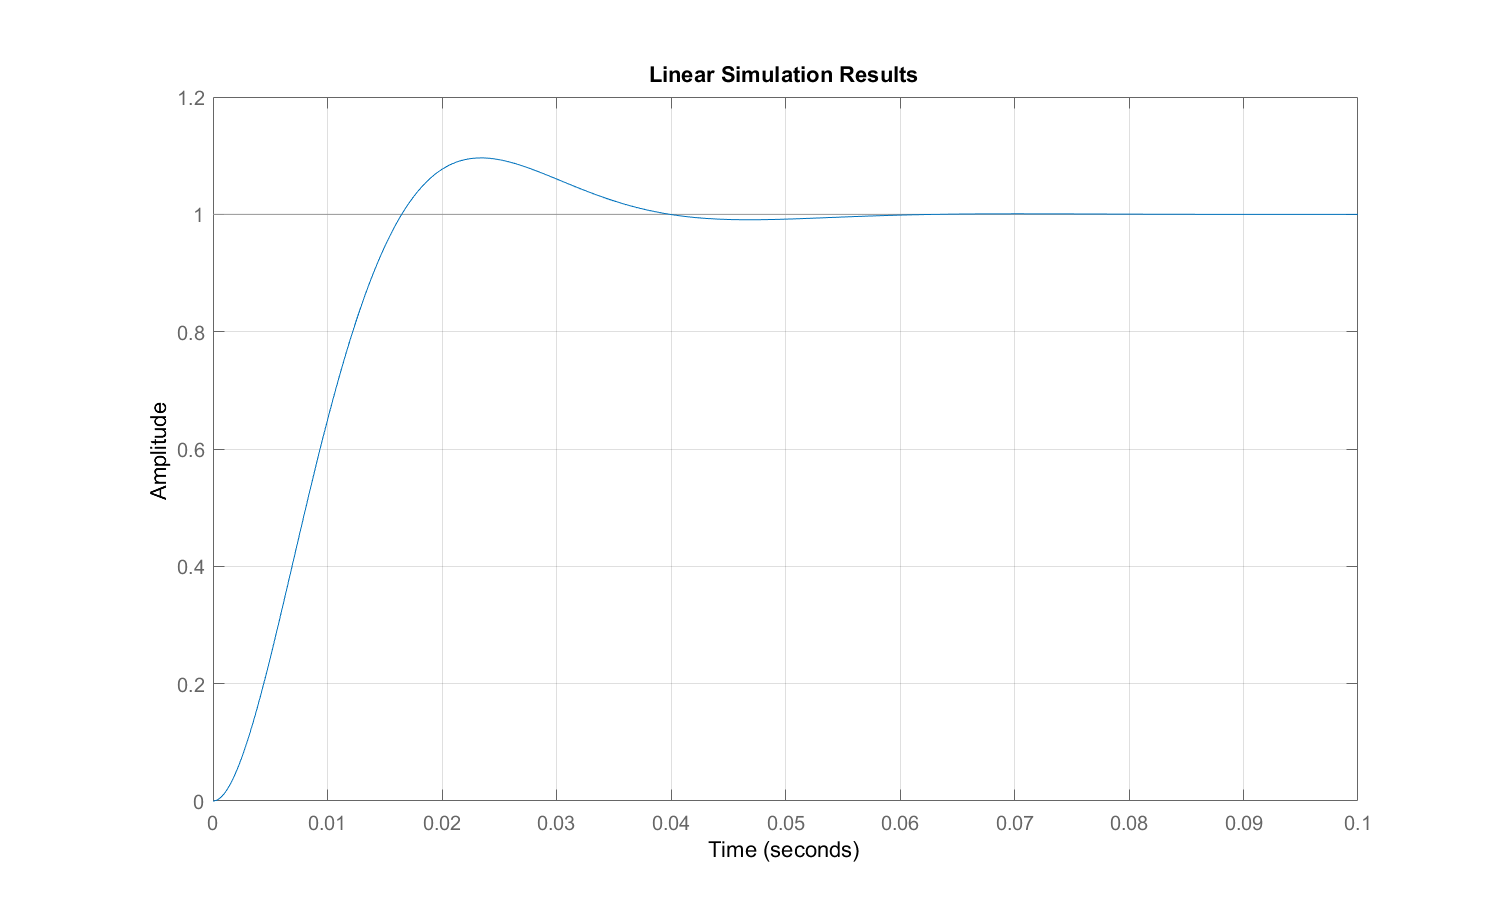
\includegraphics[scale=0.35,page=1]{ПП_№6(1).png}
	
	В данном случае время регулирования $t_{\text{р}} = 0.03$ с, перерегулирование $\sigma_{\max} = 10 \%$, частота среза $\ds \omega_{\text{с}} = 140$.
	$\\$
	
	Для определения корректирующего устройства $\ds W_{\text{к}}(s)$ можно построить ЛАЧХ, содержащую $\ds L_{\text{н}}(\omega)$ для неизменяемой системы (красный цвет), $\ds L_{\text{ж}}(\omega)$ для желаемой системы (синий цвет) и $\ds L_{\text{к}}(\omega) = L_{\text{ж}}(\omega) - L_{\text{н}}(\omega)$ для корректирующего устройства (зелёный цвет).
	
	\begin{center}
		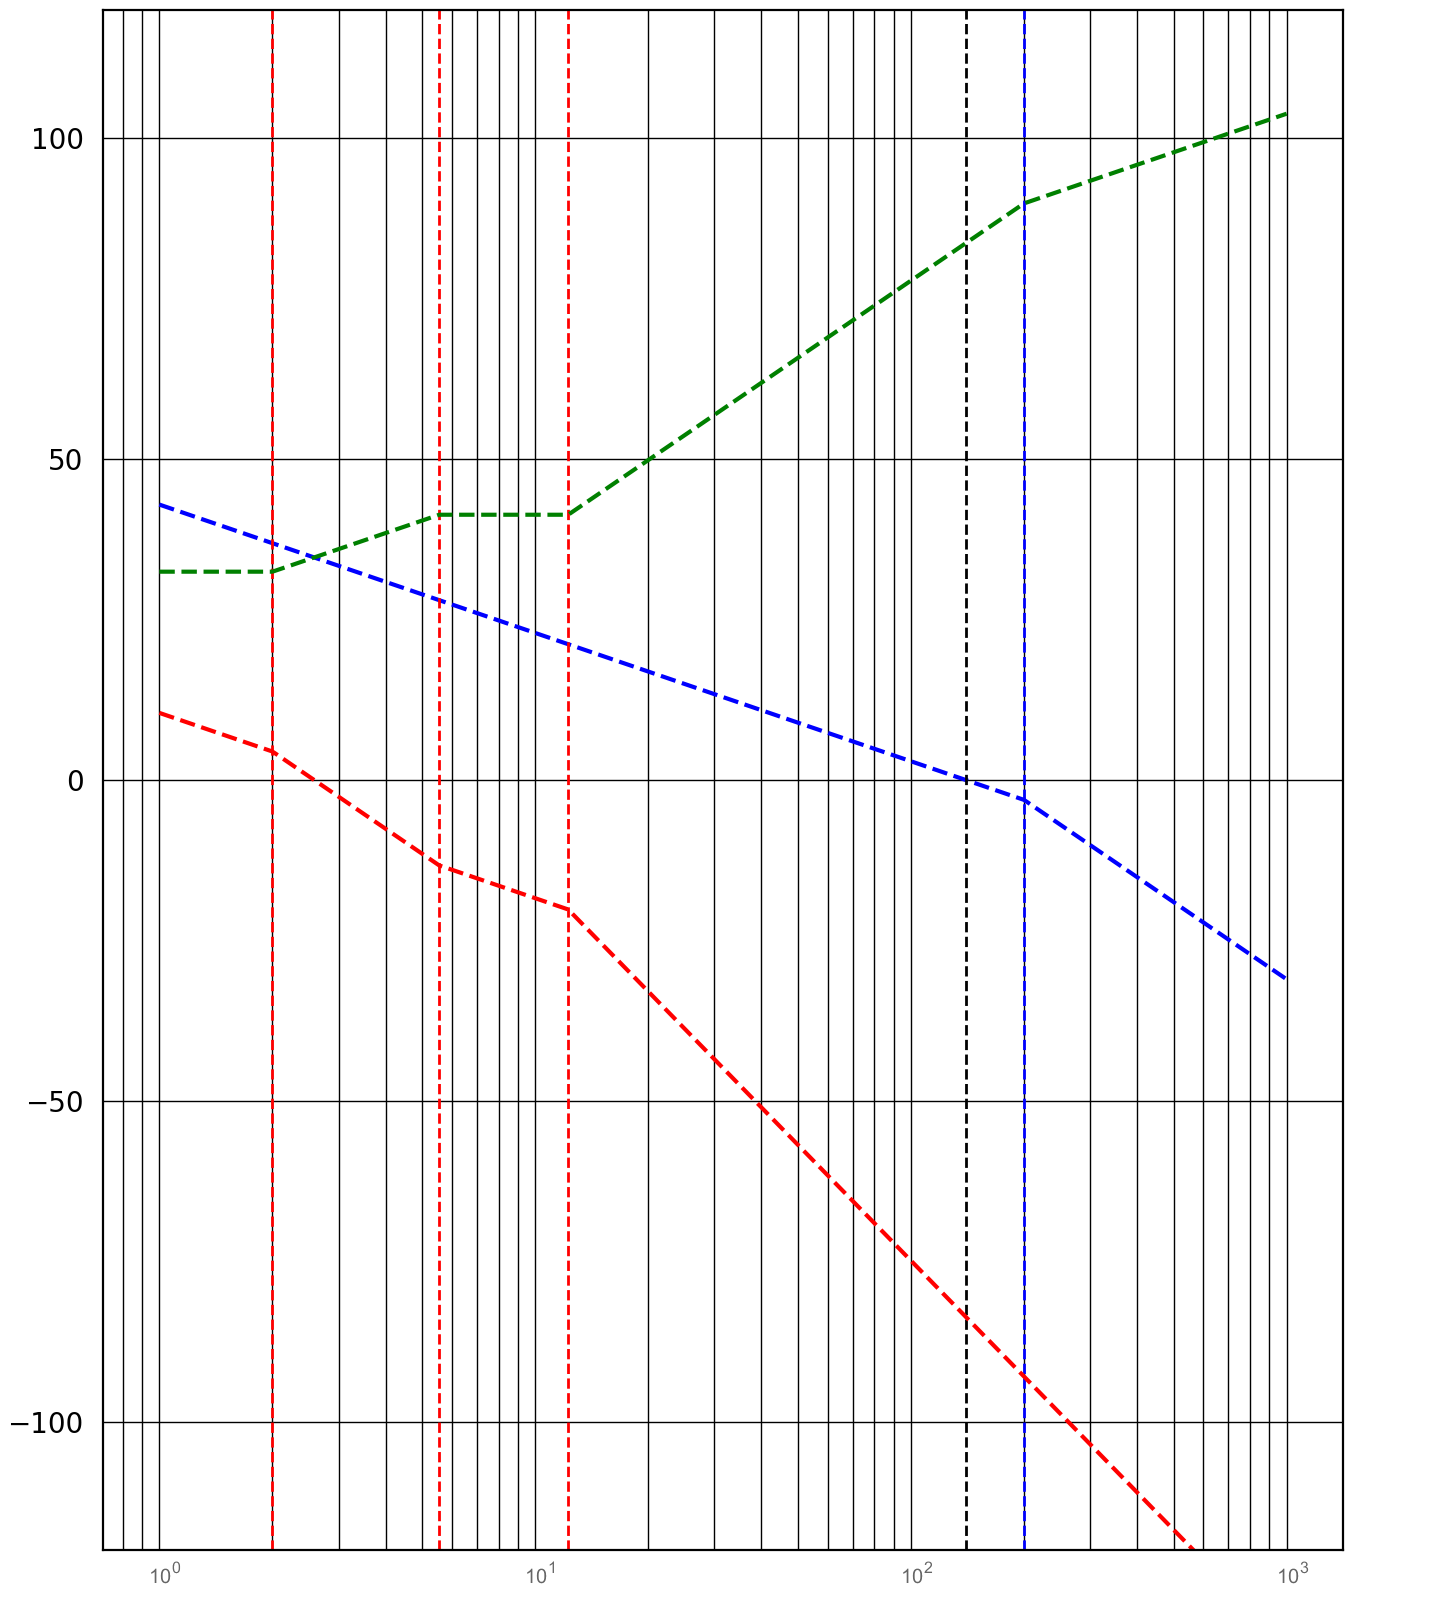
\includegraphics[scale=0.85,page=1]{ЛАЧХ_6(1).png}
	\end{center}

	Получаем:
	
	$\ds W_{\text{к}}(s) = 42 \; (1 + 0.5 s) \; \bigg( 1 + \frac{5}{90} s + \frac{2}{300} s^2 \bigg) \; \frac{1}{0.005 s + 1} \; \frac{1}{0.18 s + 1}$
	\vs
	
	Поскольку здесь степень числителя превосходит степень знаменателя на единицу, нужно добавить апериодическое звено $\ds \frac{1}{0.0001 s + 1}$, которое не вносит значимых изменений в систему при частотах ниже $10^4$. Итак:
	\vs
	
	$\ds W_{\text{к}}(s) = 42 \; (1 + 0.5 s) \; \bigg( 1 + \frac{5}{90} s + \frac{2}{300} s^2 \bigg) \; \frac{1}{0.005 s + 1} \; \frac{1}{0.18 s + 1}  \; \frac{1}{0.0001 s + 1}$
	
	\newpage
	
	Переходный процесс при действии единичного ступенчатого воздействия для скорректированной системы:
	
	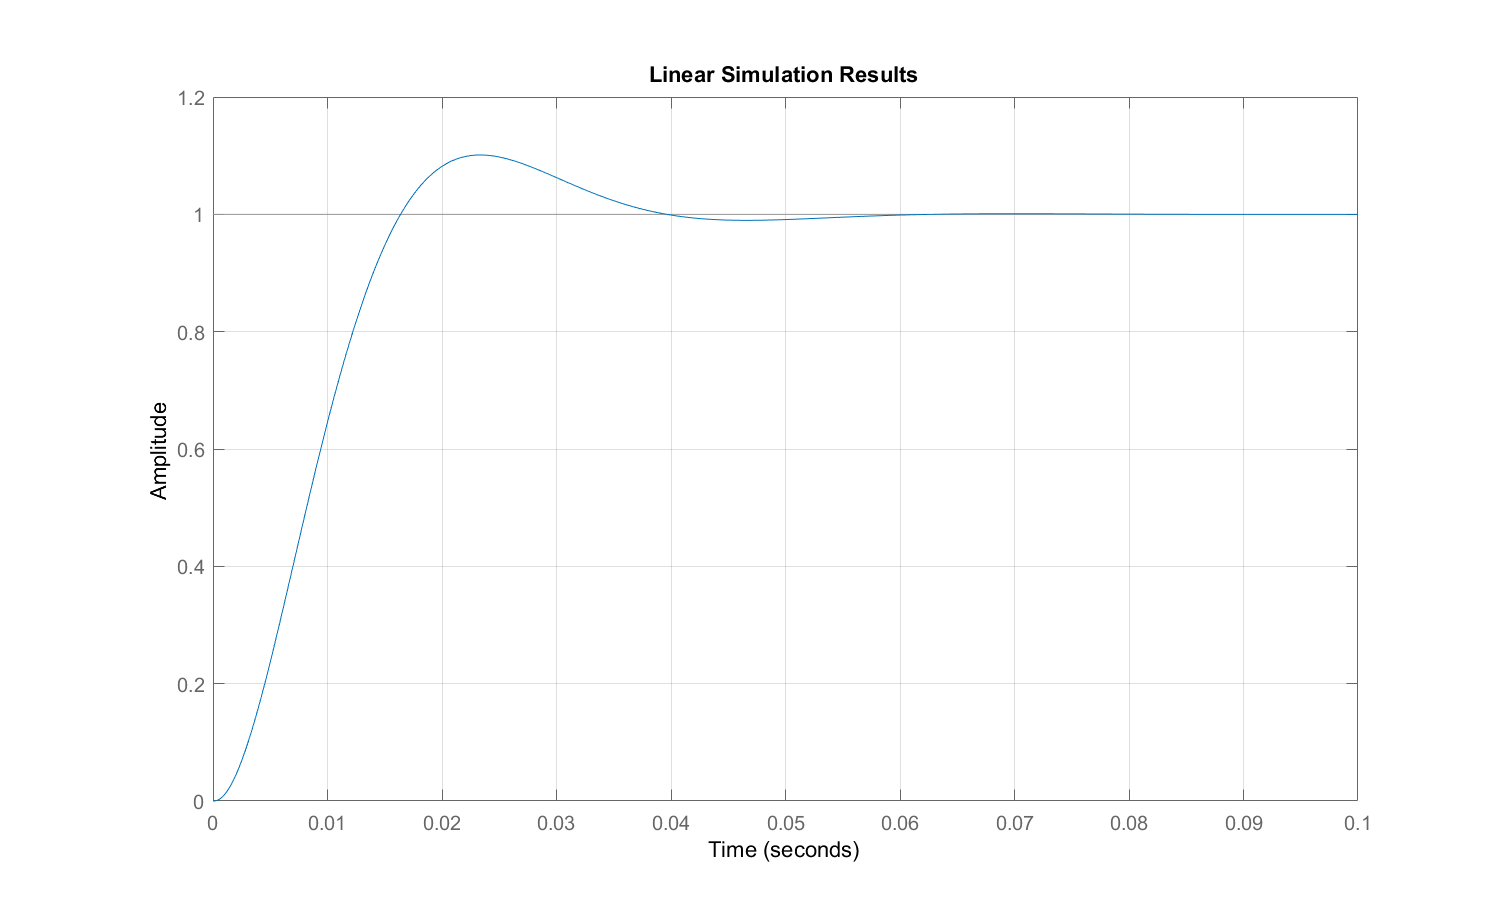
\includegraphics[scale=0.35,page=1]{ПП_№6(2).png}
	
	В данном случае время регулирования $t_{\text{р}} = 0.03$ с, перерегулирование $\sigma_{\max} = 10 \%$.
	
	
	
\end{document}